\subsection{Einleitung}
% --------------------------------------------------
\begin{frame}
  \frametitle{Das \znull-Teilchen}
  \begin{columns}
    \begin{column}{0.6\textwidth}
      \centering
      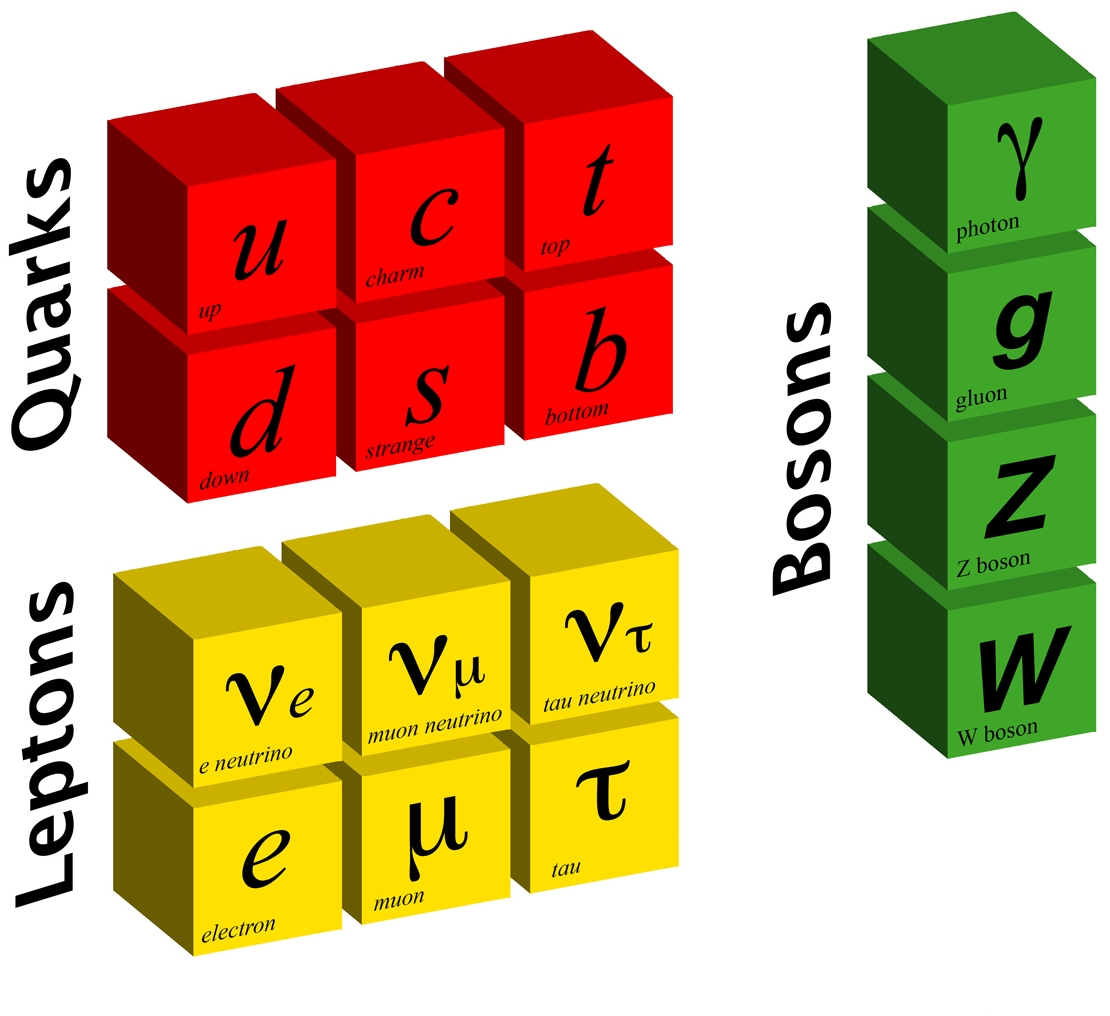
\includegraphics[width=0.8\textwidth]{sm/sm_blocks_wo_higgs.jpg}
    \end{column}
    \begin{column}{0.4\textwidth}
      \begin{block}{\znull-Teilchen}
        \begin{itemize}
        \item Austauschteilchen der Schwachen Kraft
        \item Elektrisch neutral
        \item 90 mal schwerer als das Proton
        \item Umwandlung (``Zerfall'') in leichtere Teilchen nach $3\cdot10^{-25}\sec$
        \end{itemize}
      \end{block}
    \end{column}
  \end{columns}
\end{frame}

% --------------------------------------------------
\begin{frame}
  \frametitle{In welche Teilchen zerf\"allt das \znull?}
  Es m\"ussen bestimmte Bedingungen erf\"ullt sein:
  \vskip0.5cm
  \begin{columns}
    \visible<2->{
      \begin{column}{0.48\textwidth}
        \begin{block}{Ladungserhaltung}
          \centering
          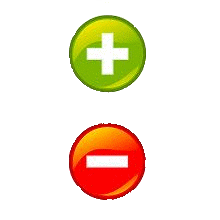
\includegraphics[height=0.2\textheight]{z0measurement/PlusMinus.png}
          \begin{itemize}
          \item Zerfallsprodukte m\"ussen Ladung 0 haben
          \item<3-> \znull zerf\"allt in Teilchen-Antiteilchen-Paar
          \item<3-> Z.B.\ $\znull\rightarrow e^{+}e^{-}$
          \end{itemize}
        \end{block}
      \end{column}
    }
    \visible<4->{    
      \begin{column}{0.04\textwidth}
      \end{column}
      \begin{column}{0.48\textwidth}
        \begin{block}{Energie- und Impulserhaltung}
          \centering
          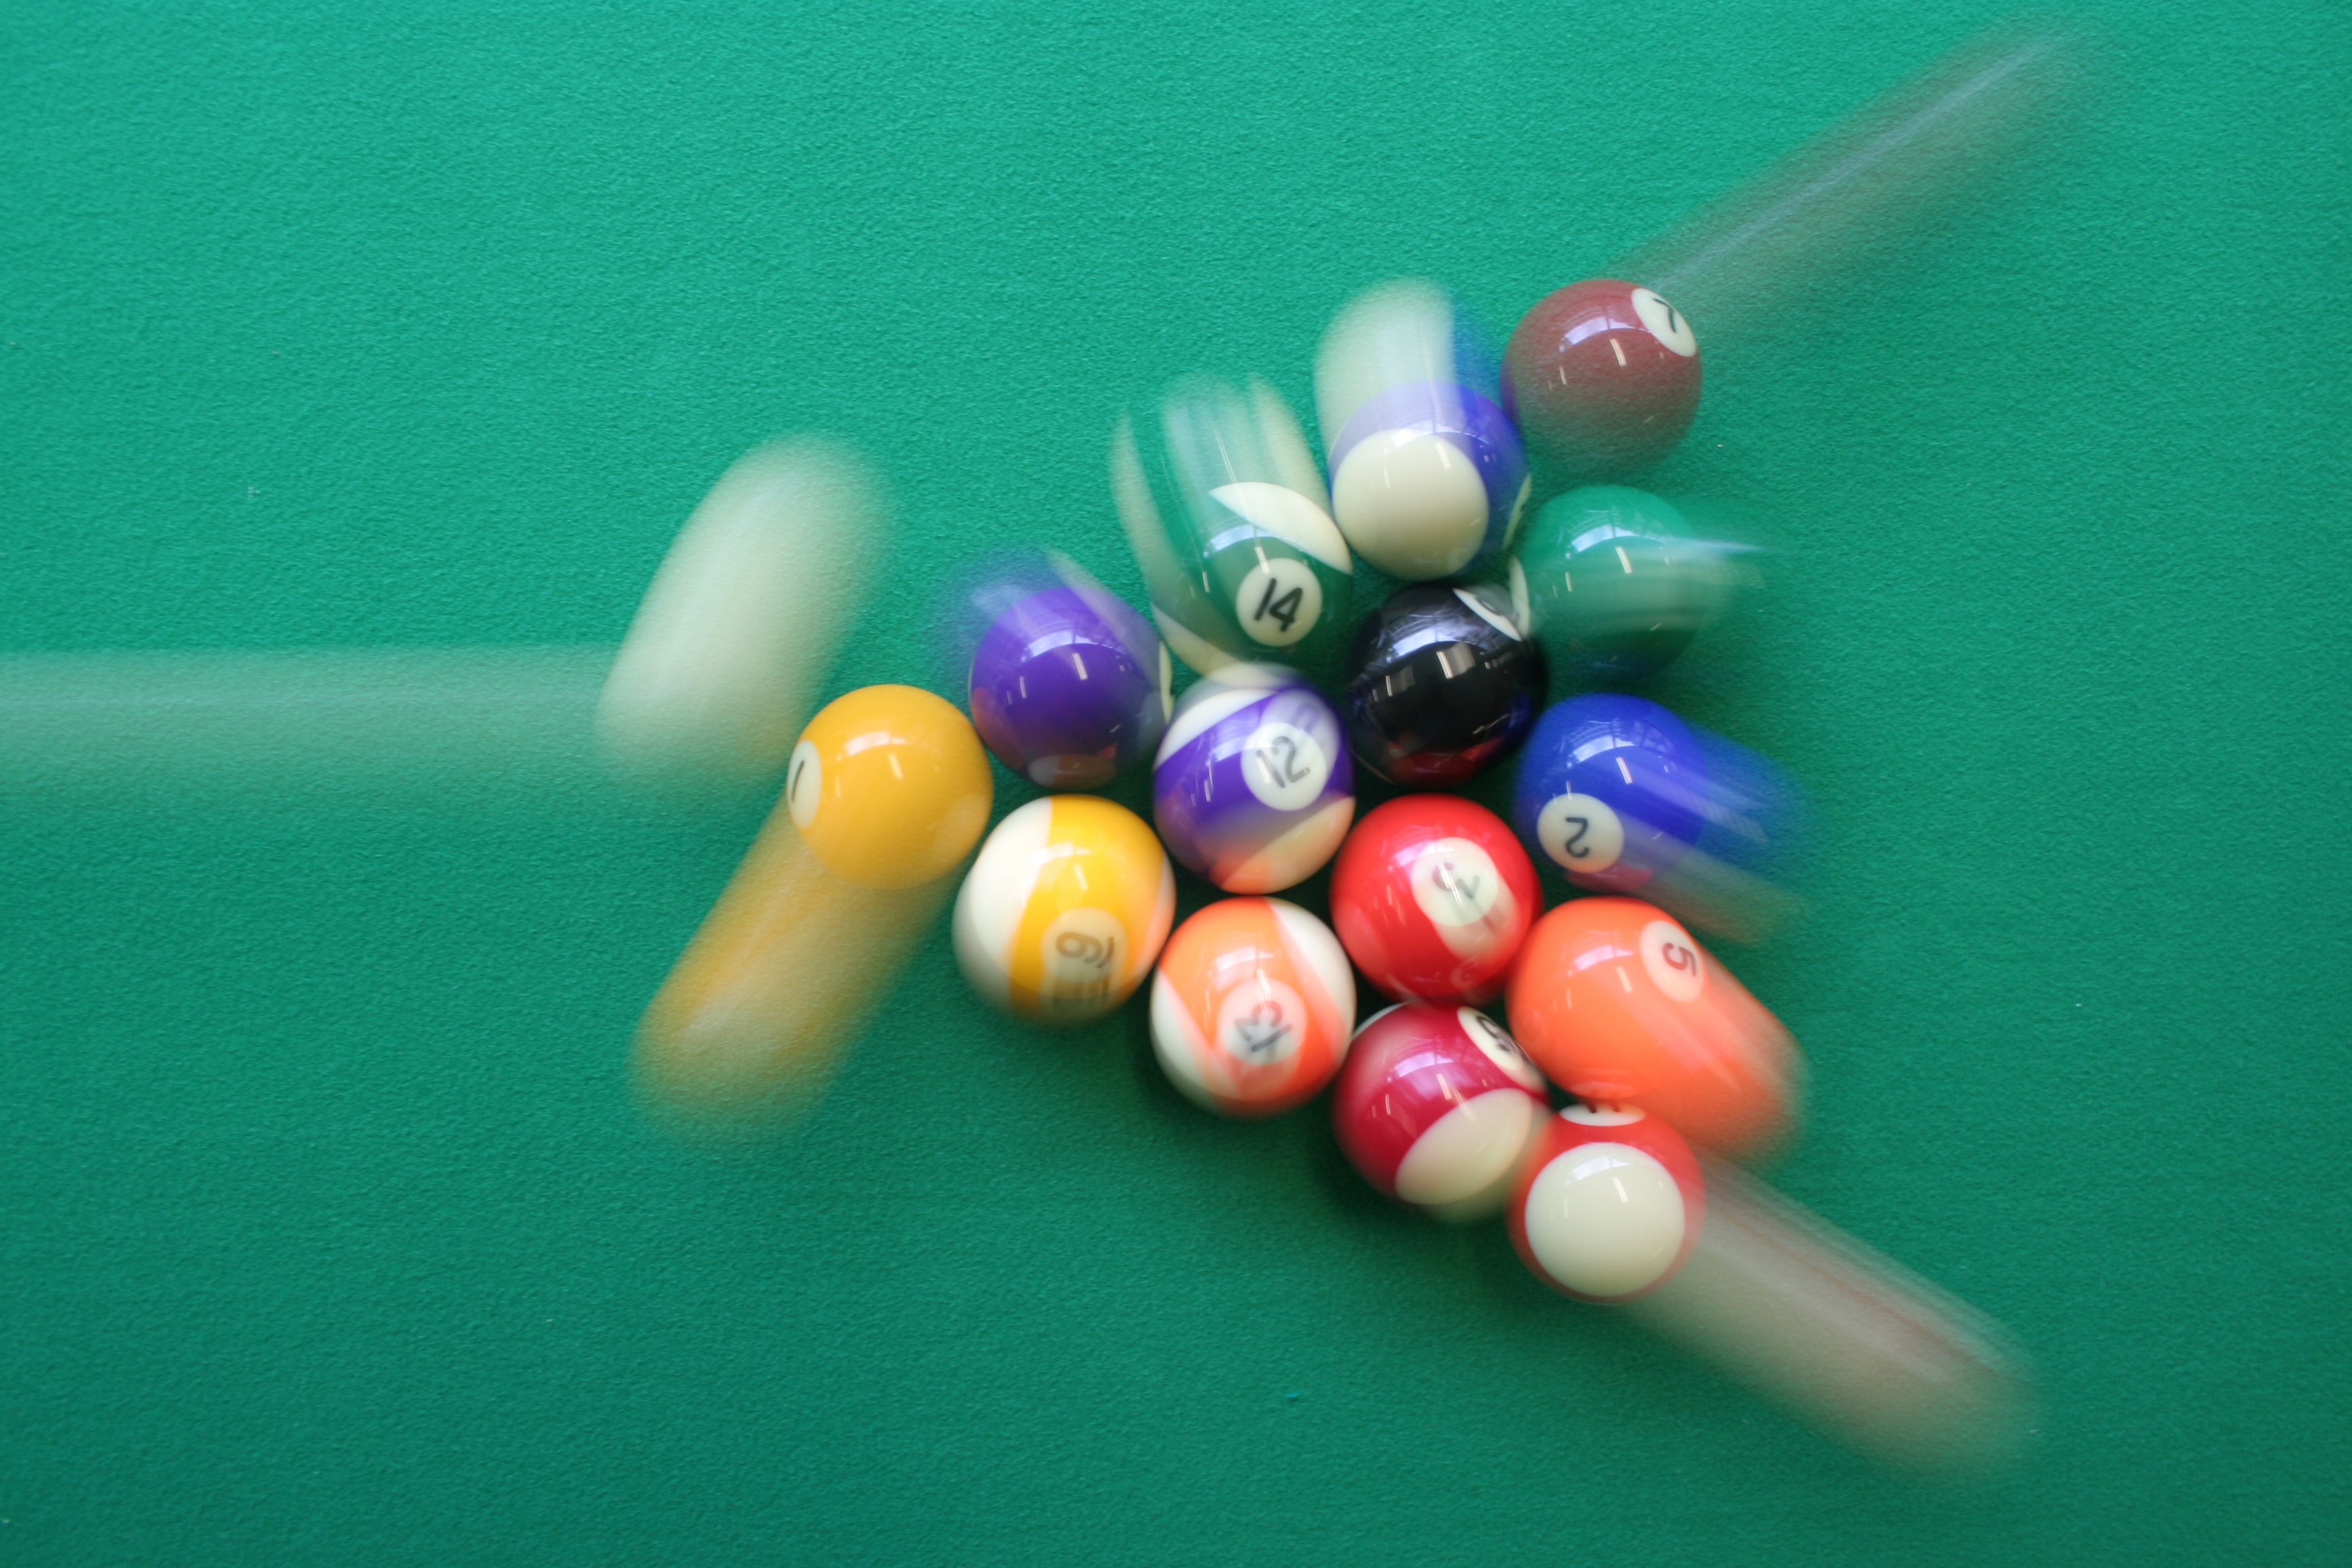
\includegraphics[rotate=90,height=0.2\textheight]{z0measurement/Impulserhaltung_Billard.jpg}
          \begin{itemize}
          \item<5-> Teilchen und Antiteilchen bewegen sich in
            entgegengesetzte Richtung
          \item<5-> Beide haben die gleiche Energie
          \end{itemize}
        \end{block}
      \end{column}
    }
  \end{columns}
\end{frame}

% --------------------------------------------------
\begin{frame}[t]
  \frametitle{In welche Teilchen zerf\"allt das \znull?}
  \vskip-0.4cm
  \begin{columns}[T]
    \begin{column}{0.5\textwidth}
      \centering
      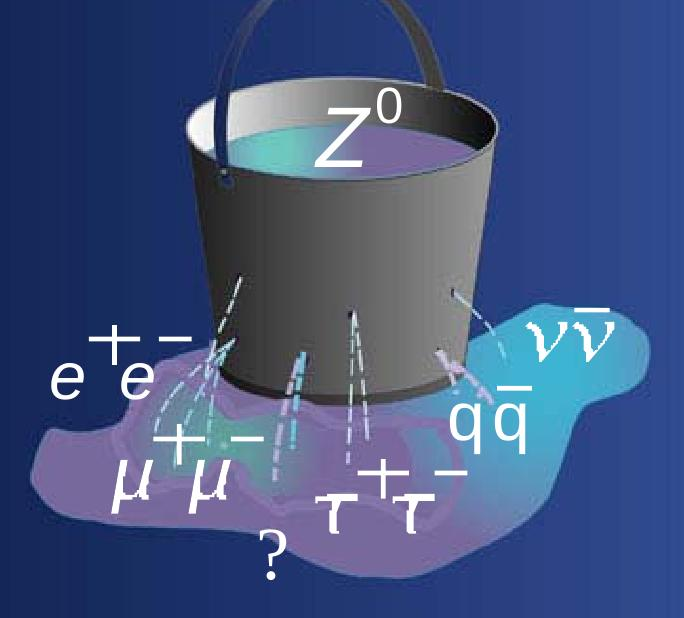
\includegraphics[height=0.37\textheight]{z0measurement/Z0_bucket.jpg}
      \vskip0.1cm
      \begin{itemize}
      \item Wasser kann durch verschiedene L\"ocher ausflie\ss{}en
        \textcolor{white}{(``Zerfallskan\"ale'')}
      \item[~] \textcolor{white}{ F\"ur ein bestimmtes Molek\"ul Loch nicht vorhersagbar}
      \item[~] \textcolor{white}{ Verh\"altnis der Austrittsmengen $\propto$ Gr\"o\ss{}e der
          L\"ocher}
      \end{itemize}
    \end{column}
    \begin{column}{0.5\textwidth}
    \end{column}
  \end{columns}
\end{frame}

% --------------------------------------------------
\begin{frame}[t]
  \frametitle{In welche Teilchen zerf\"allt das \znull?}
  \vskip-0.4cm
  \begin{columns}[T]
    \begin{column}{0.5\textwidth}
      \centering
      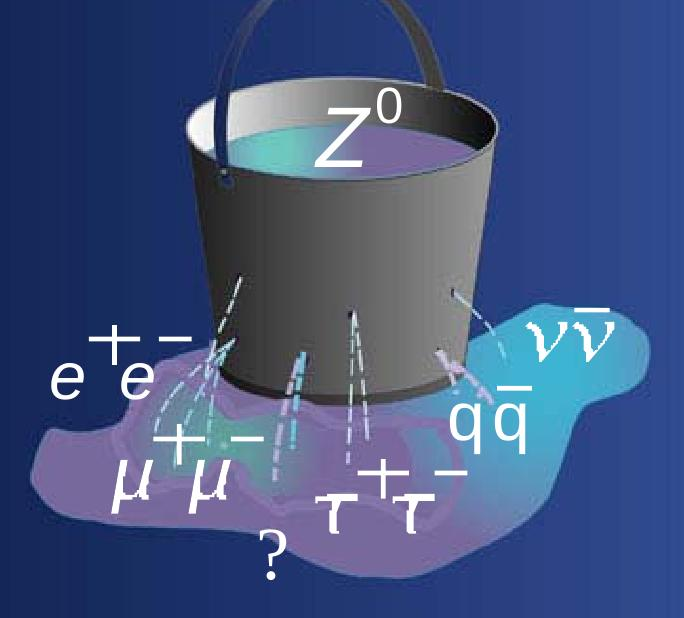
\includegraphics[height=0.37\textheight]{z0measurement/Z0_bucket.jpg}
      \vskip0.1cm
      \begin{itemize}
      \item<1-> Wasser kann durch verschiedene L\"ocher ausflie\ss{}en \textcolor{white}{(``Zerfallskan\"ale'')}
      \item<2-> F\"ur ein bestimmtes Molek\"ul Loch nicht vorhersagbar
      \item<3-> Verh\"altnis der Austrittsmengen $\propto$ Gr\"o\ss{}e der
        L\"ocher
      \end{itemize}
    \end{column}
    \begin{column}{0.5\textwidth}
      \centering
      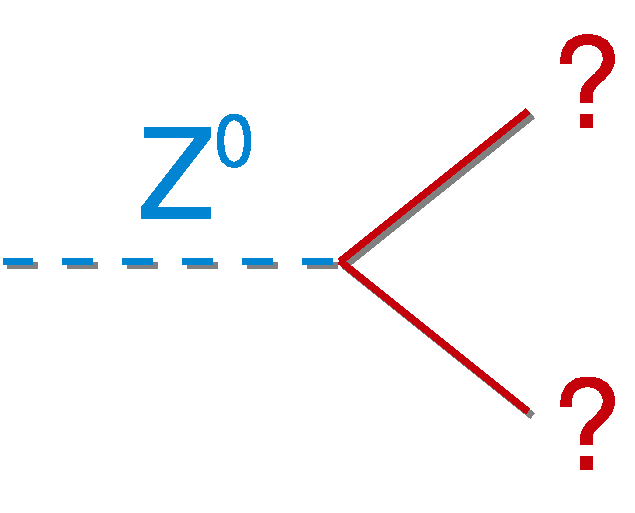
\includegraphics[height=0.37\textheight]{z0measurement/Z0-Feynman_anything.pdf}
      \begin{itemize}
      \item<1-> \znull kann in verschiedene Teilchen-Antiteilchen-Paare (``Zerfallskan\"ale'')
        zerfallen
      \item<2-> F\"ur ein bestimmtes \znull Zerfallskanal nicht vorhersagbar
      \item<3-> Verh\"altnis der Zerfallsh\"aufigkeiten $\propto$ St\"arke der Kopplungen
      \end{itemize}
    \end{column}
  \end{columns}
\end{frame}

% --------------------------------------------------
 \begin{frame}
   \frametitle{Unsere Aufgabe}
   \begin{block}{}
     \begin{columns}
       \begin{column}{0.2\textwidth}
         \centering
         
\includegraphics[height=0.2\textheight]{eyecandy/Sheldon}
       \end{column}
       \begin{column}{0.8\textwidth}
         ``Wie h\"aufig zerf\"allt das \znull \"uber welchen Kanal?''
       \end{column}
     \end{columns}
   \end{block}
   \vskip1cm
   \begin{columns}
     \begin{column}{0.4\textwidth}
       \centering
       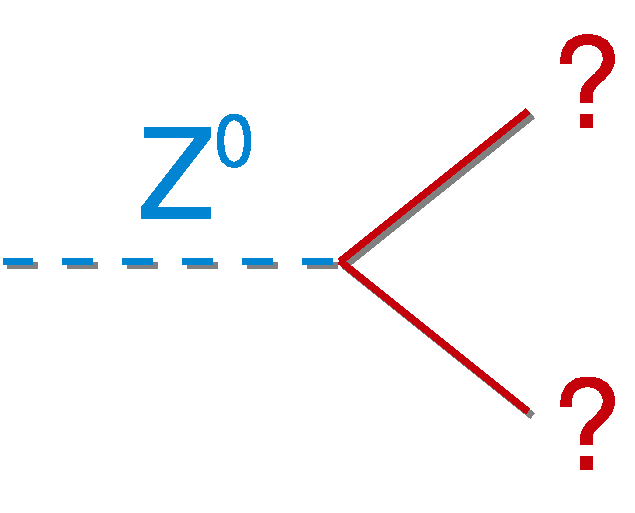
\includegraphics[width=0.9\textwidth]{z0measurement/Z0-Feynman_anything.pdf}
     \end{column}
     \begin{column}{0.05\textwidth}
     \end{column}
     \begin{column}{0.55\textwidth}
       \pause
       \begin{block}{Wir betrachten vier Zerfallskan\"ale}
         \begin{itemize}
         \item $\znull\rightarrow e^{+}e^{-}$
         \item $\znull\rightarrow \mu^{+}\mu^{-}$
         \item $\znull\rightarrow \tau^{+}\tau^{-}$
         \item $\znull\rightarrow q\bar{q}$
         \end{itemize}
       \end{block}
    \end{column}
  \end{columns}
 \end{frame}

 \subsection{OPAL}
 % --------------------------------------------------
 \begin{frame}
   \frametitle{Woher bekommen wir die Daten?}
   \begin{block}{Large Electron Positron Collider (LEP)}
     \begin{columns}[T]
       \begin{column}{0.6\textwidth}
         \begin{itemize}
         \item $e^{+}e^{-}$-Beschleuniger
        \item Vier gro\ss{}e Experimente
           \begin{itemize}
           \item ALEPH, Delphi, L3 und OPAL
           \end{itemize}
         \end{itemize}
       \end{column}
       \begin{column}{0.4\textwidth}
         \vskip-0.5cm
         \centering
         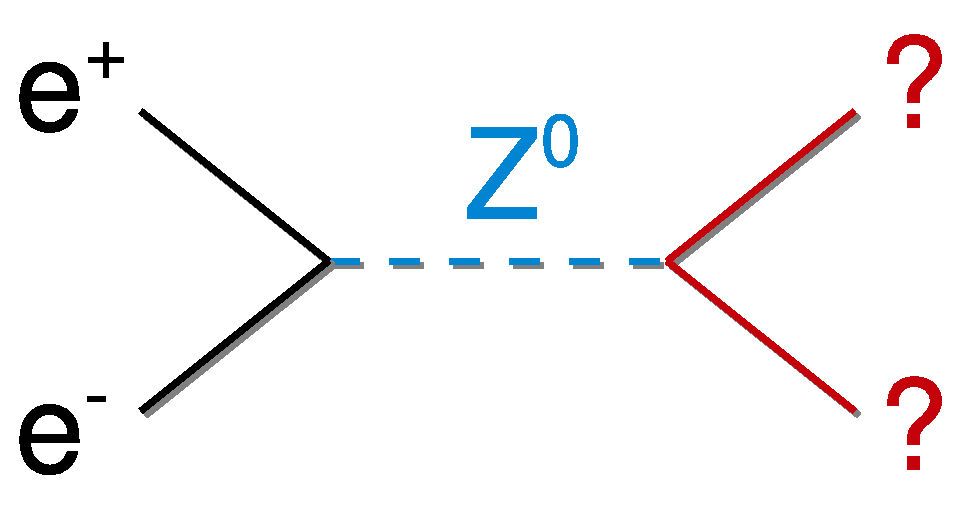
\includegraphics[width=0.9\textwidth]{z0measurement/Z0-Feynman_LEP}
       \end{column}
     \end{columns}
   \end{block}
   \pause
   \begin{block}{Omni Purpose Apparatus at LEP (OPAL)}
     \begin{columns}
       \begin{column}{0.6\textwidth}
         \begin{itemize}
         \item Betrieb von 1989 bis 2000 am CERN
         \item Wichtige Aufgabe
           \begin{itemize}
           \item Genaue Vermessung der \znull-Zerfallsprodukte
           \end{itemize}
         \end{itemize}
       \end{column}
       \begin{column}{0.4\textwidth}
         \vskip-0.5cm
         \centering
         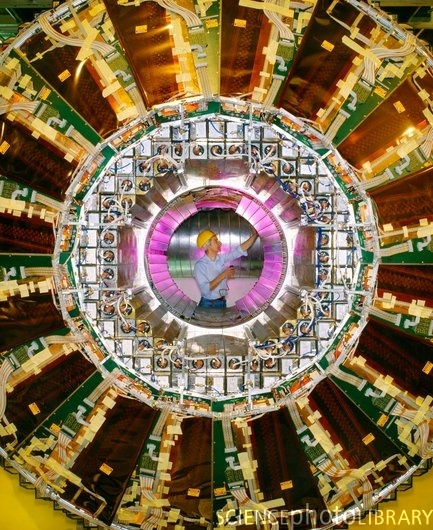
\includegraphics[width=0.5\textwidth]{z0measurement/A105130-The_OPAL_detector_at_CERN-SPL}
       \end{column}
     \end{columns}
   \end{block}
 \end{frame}

 % --------------------------------------------------
 \begin{frame}
   \frametitle{Der OPAL-Detektor}
   \begin{center}
     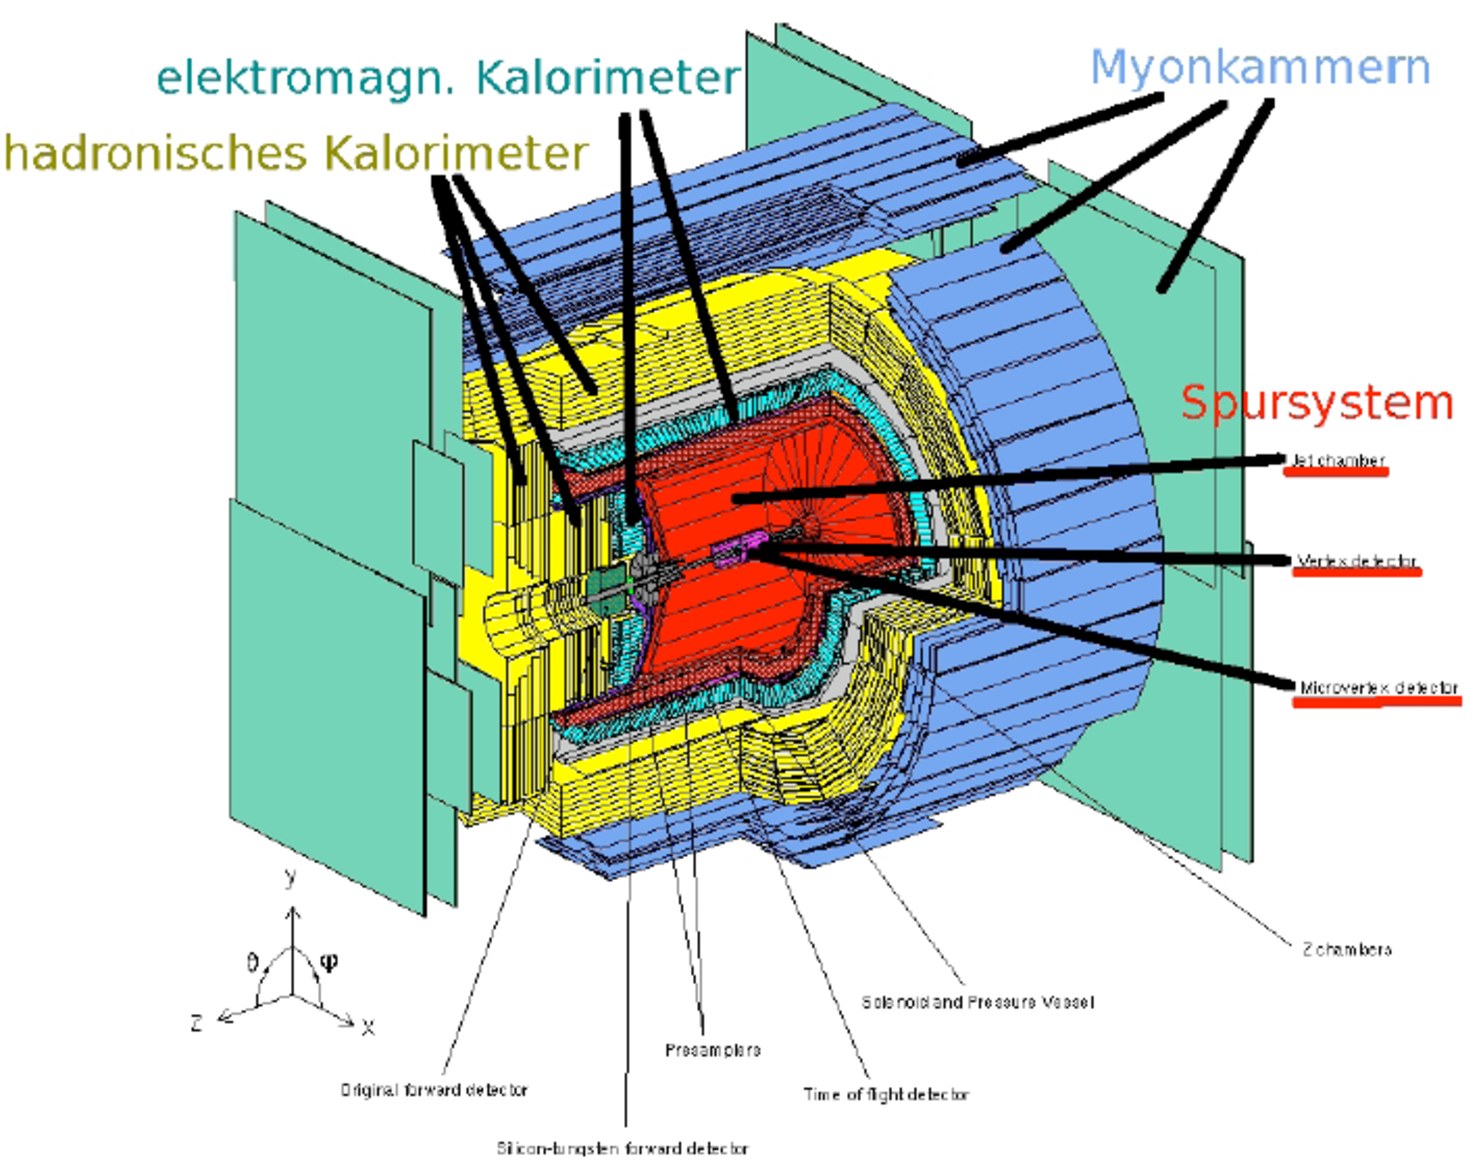
\includegraphics[width=0.8\textwidth]{z0measurement/OpalDetector}
   \end{center}
 \end{frame}

 \subsection{Teilchensignaturen}
 % --------------------------------------------------
 \begin{frame}
   \frametitle{Was sehen wir denn nun im Detektor?}
   \alert{Beispiel Elektron}: Sicht in den Detektor in Richtung Strahlachse
   \visible<1->{
     \vskip0.5cm
     \begin{columns}[T]
       \begin{column}{0.5\textwidth}
         \centering
         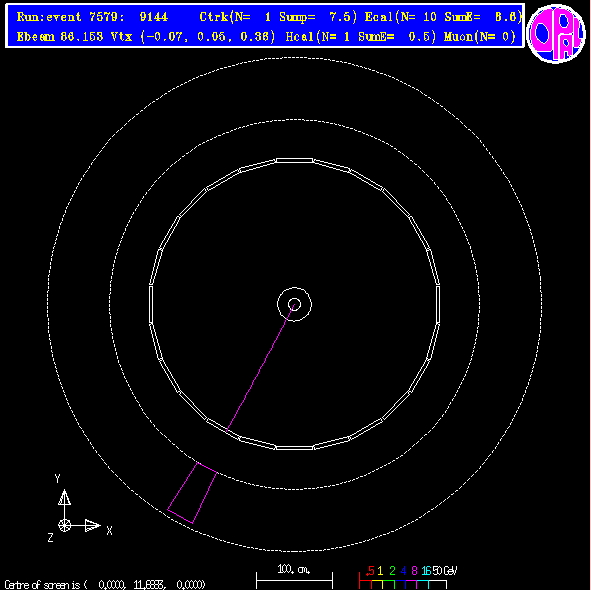
\includegraphics[width=0.9\textwidth]{opalevents/ex_electron}\\
         Frontalansicht
       \end{column}
       \begin{column}{0.5\textwidth}
         \visible<2->{
           \begin{enumerate}
           \item<3-> Spur im Spurdetektor (\textcolor{magenta}{---})
             \begin{center}
               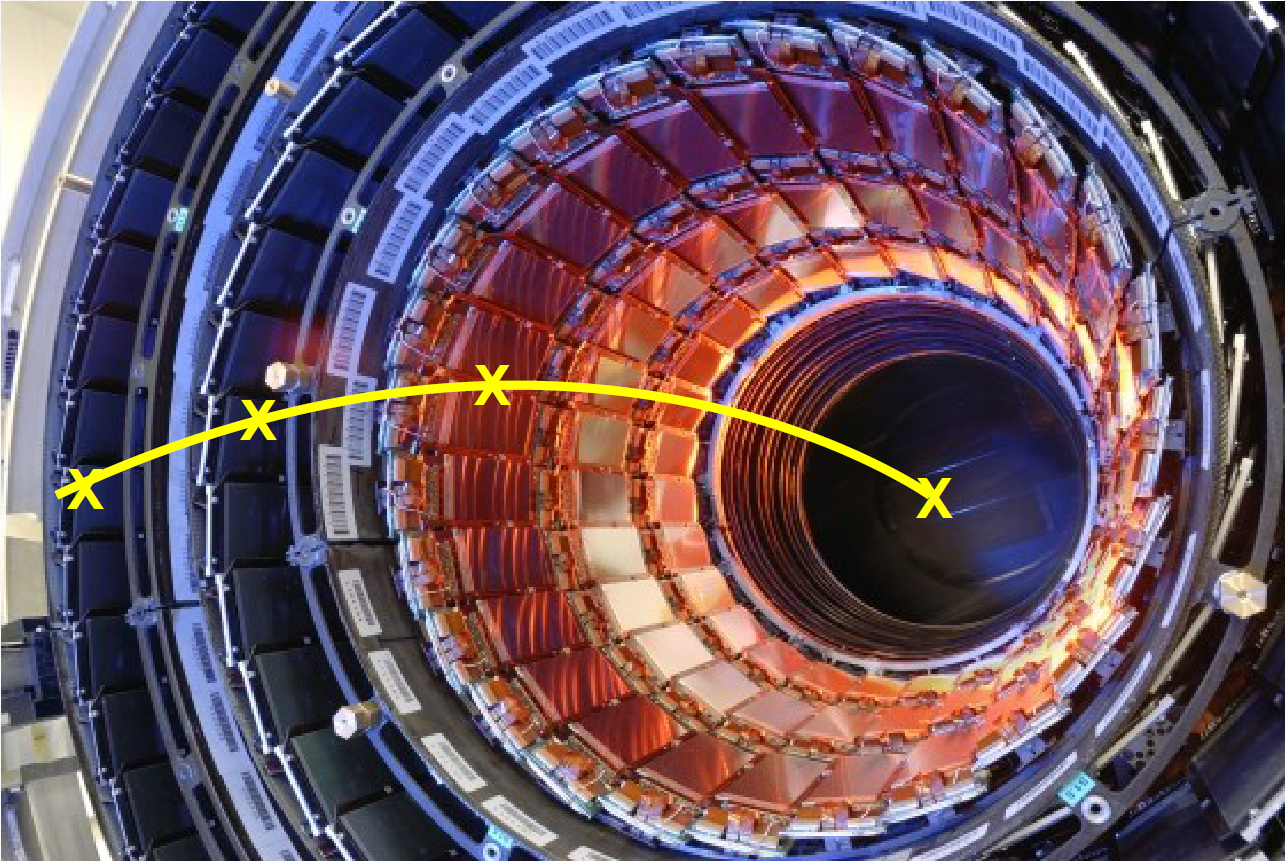
\includegraphics[width=0.6\textwidth]{lhc/Tracker_Hits_Track.png}
             \end{center}
           \item<4-> Energie im elektromagnetischen Kalorimeter (\textcolor{red}{$\square$})
             \begin{center}
               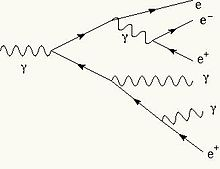
\includegraphics[width=0.6\textwidth]{lhc/220px-Schematic_of_a_particle_shower}
             \end{center}
           \end{enumerate}
         }
       \end{column}
     \end{columns}
   }
 \end{frame}

 % --------------------------------------------------
 \begin{frame}
   \frametitle{Signatur eines Elektrons}
   \begin{columns}
     \begin{column}{0.5\textwidth}
       \centering
       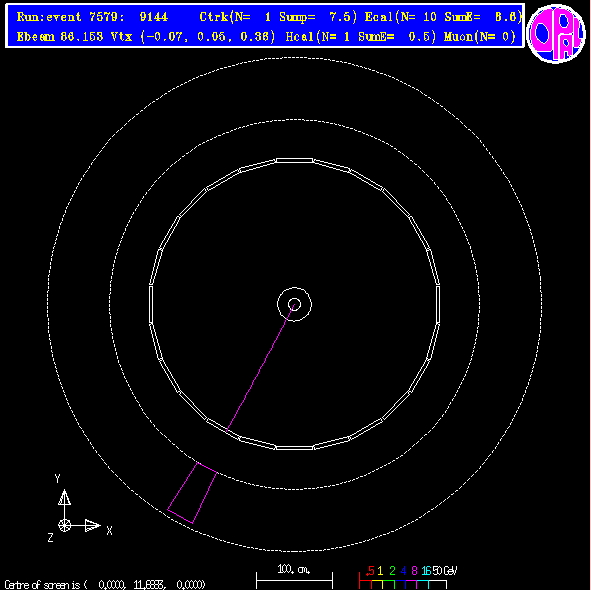
\includegraphics[width=0.95\textwidth]{opalevents/ex_electron}\\
       Frontalansicht
     \end{column}
     \begin{column}{0.5\textwidth}
       \centering
       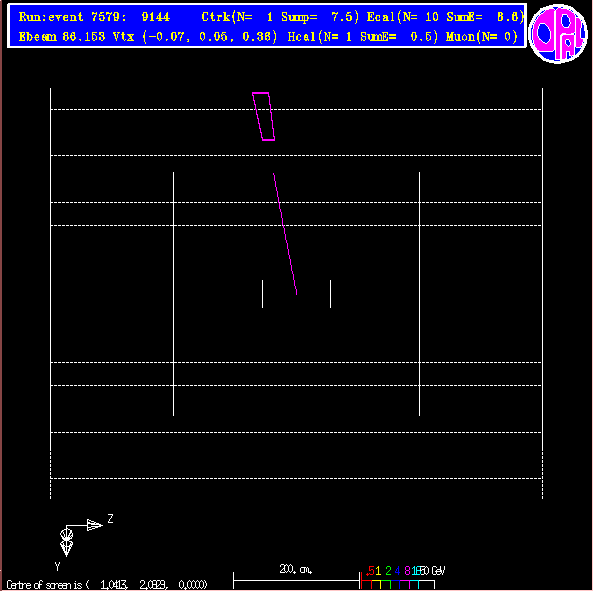
\includegraphics[width=0.95\textwidth]{opalevents/ex_electron_z}\\
       Seitenansicht
     \end{column}
  \end{columns}
 \end{frame}

 \subsection{Zerf\"alle im OPAL-Detektor}
 % --------------------------------------------------
 \begin{frame}
   \frametitle{Eure Aufgabe}
   \begin{columns}
     \begin{column}{0.15\textwidth}
     \end{column}
     \begin{column}{0.7\textwidth}
       \begin{block}{Untersucht die Ereignisbilder von \znull-Zerf\"allen}
         \begin{itemize}
         \item In welche Teilchen ist das \znull zerfallen?
         \item Wie oft kommt welcher Zerfallskanal vor?
         \item Stimmt die Theorie?
         \end{itemize}
       \end{block}
     \end{column}
     \begin{column}{0.15\textwidth}
     \end{column}
   \end{columns}
   \pause
   \vskip1.5cm
   \begin{center}
     \alert{Vorher schauen wir uns noch gemeinsam ein paar Beispiele an}
   \end{center}
 \end{frame}

 % --------------------------------------------------
 \begin{frame}
   \frametitle{Was sieht man bei einem \znull-Zerfall?}
   \begin{columns}
     \begin{column}{0.5\textwidth}
       \visible<2->{
         \begin{block}{Ladungserhaltung}
           \begin{itemize}
           \item \znull zerf\"allt in ein Teilchen-Antiteilchen-Paar
           \item Z.\,B.\ $\znull\rightarrow e^{+}e^{-}$
           \end{itemize}
         \end{block}
       }
       \visible<3->{
         \begin{block}{Energie- und Impulserhaltung}
           \begin{itemize}
           \item Teilchen und Antiteilchen bewegen sich in
             entgegengesetzte Richtung
           \item Beide haben die gleiche Energie
           \end{itemize}
         \end{block}
       }
     \end{column}
     \visible<4->{
       \begin{column}{0.5\textwidth}
         \centering
         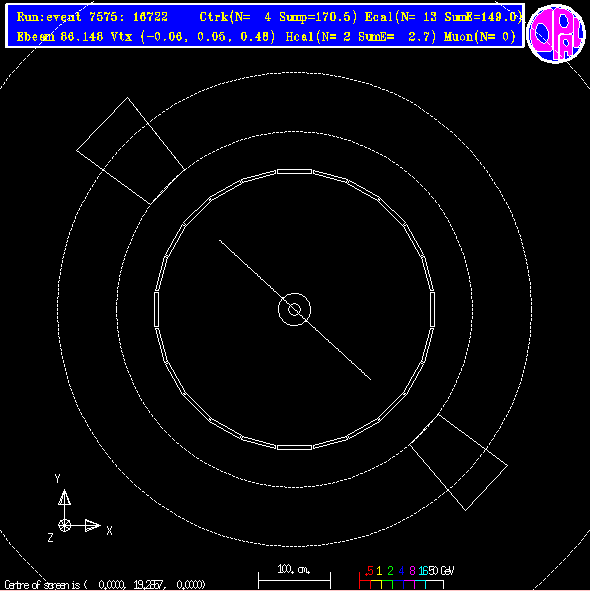
\includegraphics[width=0.95\textwidth]{opalevents/z_ee_xy}
       \end{column}
     }
   \end{columns}
   \visible<5->{
     \vskip0.5cm
     \begin{center}
       \alert{Es werden die Zerfallsprodukte und nicht das \znull direkt
         beobachtet}
     \end{center}
   }
 \end{frame}

 % --------------------------------------------------
 \begin{frame}
   \frametitle{$\znull\rightarrow\mu^{+}\mu^{-}$}
   \begin{center}
     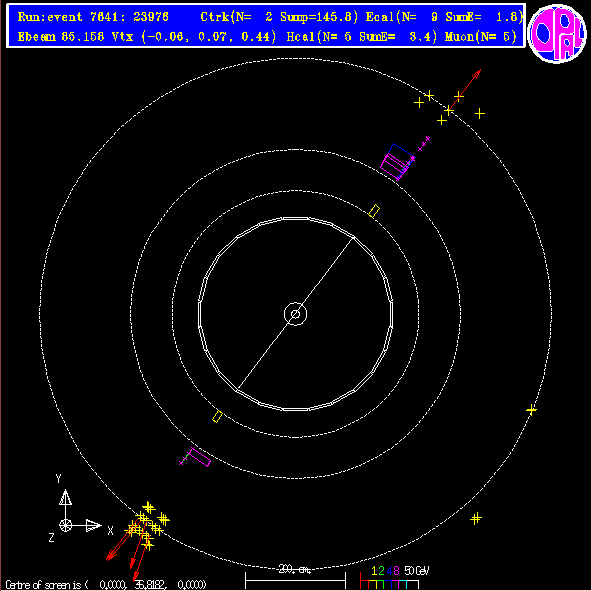
\includegraphics[width=0.5\textwidth]{opalevents/z_mumu_xy}
   \end{center}
 \end{frame}

 % --------------------------------------------------
 \begin{frame}
   \frametitle{$\znull\rightarrow q\bar{q}$}
   \pause
   \begin{columns}
     \begin{column}{0.5\textwidth}
       \begin{block}{Jets}
         \begin{itemize}
         \item Energiereiches Quark erzeugt B\"undel von Teilchen
           (``Jet'')
           \begin{center}
             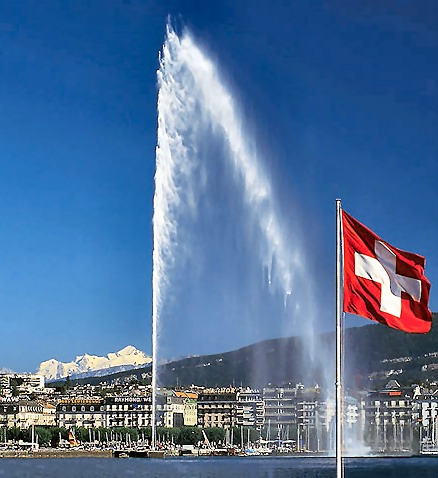
\includegraphics[width=0.4\textwidth]{z0measurement/Jetdeau}
           \end{center}
         \item Haupts\"achlich Hadronen
           \begin{itemize}
           \item<3-> Spuren im Spurdetektor
           \item<4-> Energie im elektromagnetischen und hadronischen Kalorimeter
           \end{itemize}
         \end{itemize}
       \end{block}
    \end{column}
     \begin{column}{0.5\textwidth}
       \visible<5->{
         \centering
         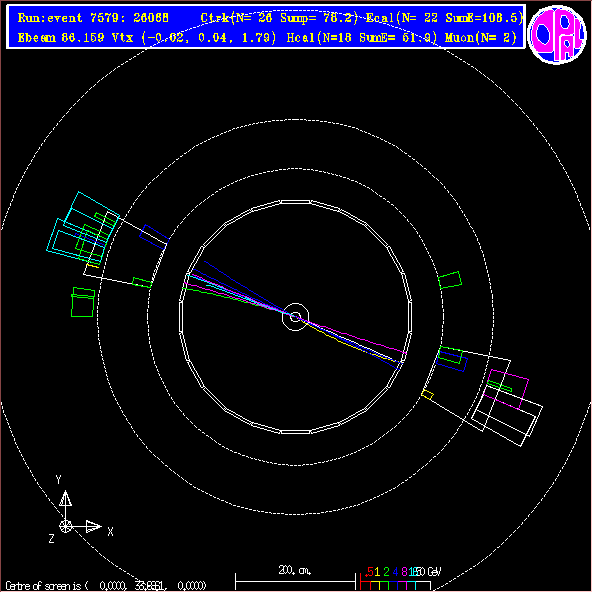
\includegraphics[width=0.95\textwidth]{opalevents/z_qq_xy}
       }
    \end{column}
   \end{columns}
   \visible<6->{
     \begin{center}
       \alert{Quarks kann man nicht direkt beobachten: $\znull\rightarrow
         q\bar{q} \rightarrow \text{Jets}$}
     \end{center}
   }
 \end{frame}
 
 % --------------------------------------------------
 \begin{frame}
   \frametitle{$\znull\rightarrow \tau^{+}\tau^{-}$}
   \begin{itemize}
   \item $\tau$ selbst sind kurzlebig
   \item Zerfall in leichtere Teilchen
   \item[$\Rightarrow$] Auch $\tau$ kann man nur indirekt beobachten!
   \end{itemize}
   \pause
   \begin{block}{M\"ogliche $\tau$-Zerf\"alle}
     \begin{columns}
       \begin{column}{0.5\textwidth}
         \begin{itemize}
           \pause
         \item $\tau \rightarrow \alert{e} + X$
           \pause
         \item $\tau \rightarrow \alert{\mu} + X$
        \end{itemize}
       \end{column}
       \begin{column}{0.5\textwidth}
         \begin{itemize}
           \pause
         \item $\tau \rightarrow \alert{\text{Jet }(1h^{\pm})} + X$
           \pause
         \item $\tau \rightarrow \alert{\text{Jet }(3h^{\pm})} + X$
         \end{itemize}
       \end{column}
     \end{columns}
   \end{block}
   \pause
   \vskip0.5cm
   \begin{columns}
     \begin{column}{0.2\textwidth}
       \centering
       
\includegraphics[width=0.6\textwidth]{z0measurement/teuferl}
     \end{column}
     \begin{column}{0.8\textwidth}
       \alert{Beliebige Kombination m\"oglich f\"ur $\znull\rightarrow \tau^{+}\tau^{-}$}
     \end{column}     
   \end{columns}
 \end{frame}

 % --------------------------------------------------
 \begin{frame}
   \frametitle{Zwei m\"ogliche $\znull\rightarrow\tau^{+}\tau^{-}$ Ereignisse}
   \begin{columns}
     \begin{column}{0.5\textwidth}
      \centering
       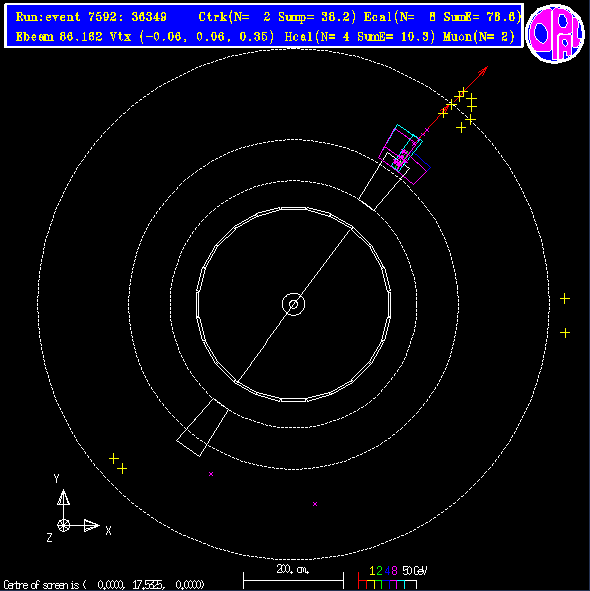
\includegraphics[width=0.9\textwidth]{opalevents/z_tautau3_xy}
       \pause
       \begin{enumerate}
       \item $\tau \rightarrow \alert{e} + X$
       \item $\tau \rightarrow \alert{\mu} + X$
       \end{enumerate}
     \end{column}
     \begin{column}{0.5\textwidth}
      \centering
      \pause
       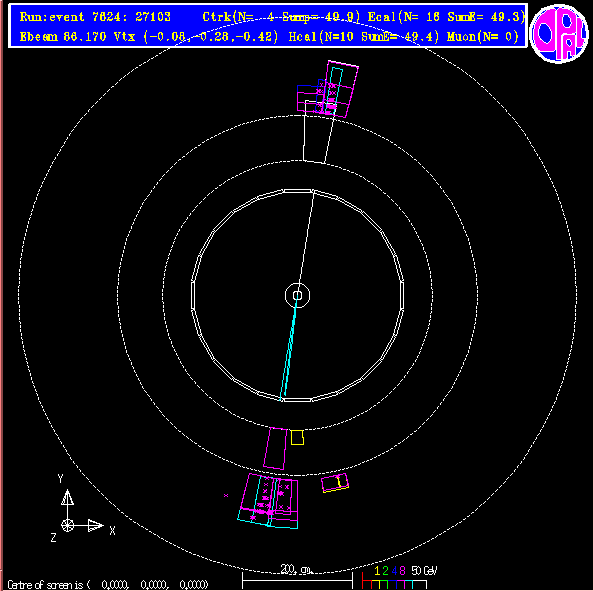
\includegraphics[width=0.9\textwidth]{opalevents/z_tautau2_xy}
       \pause
       \begin{enumerate}
       \item $\tau \rightarrow \alert{\text{Jet }(1h^{\pm})} + X$
       \item $\tau \rightarrow \alert{\text{Jet }(3h^{\pm})} + X$
       \end{enumerate}
     \end{column}
   \end{columns}
 \end{frame}

 % --------------------------------------------------
 \begin{frame}
   {\small Physics $\rightarrow$ Identifying Particles $\rightarrow$ [German] jump to measurements of Z decays}
   {\footnotesize (\url{http://physicsmasterclasses.org/exercises/manchester/de/challengez.html})}
   \vskip-0.2cm
   \begin{columns}
     \begin{column}{0.4\textwidth}
       \begin{block}{$\znull\rightarrow e^{+}e^{-}$}
         \begin{itemize}
         \item Je eine Spur und Signal im elektromagnetischen Kalorimeter
         \end{itemize}
       \end{block}
       \begin{block}{$\znull\rightarrow \mu^{+}\mu^{-}$}
         \begin{itemize}
         \item Je eine Spur, Signale in beiden Kalorimetern und Myonkammern
         \end{itemize}
       \end{block}
       \begin{block}{$\znull\rightarrow q\bar{q}$}
         \begin{itemize}
         \item Je Jets (Spuren und Signale in beiden Kalo-\\rimetern,
           manchmal $\mu$)
         \end{itemize}
       \end{block}
    \end{column}
     \begin{column}{0.6\textwidth}
       \centering
       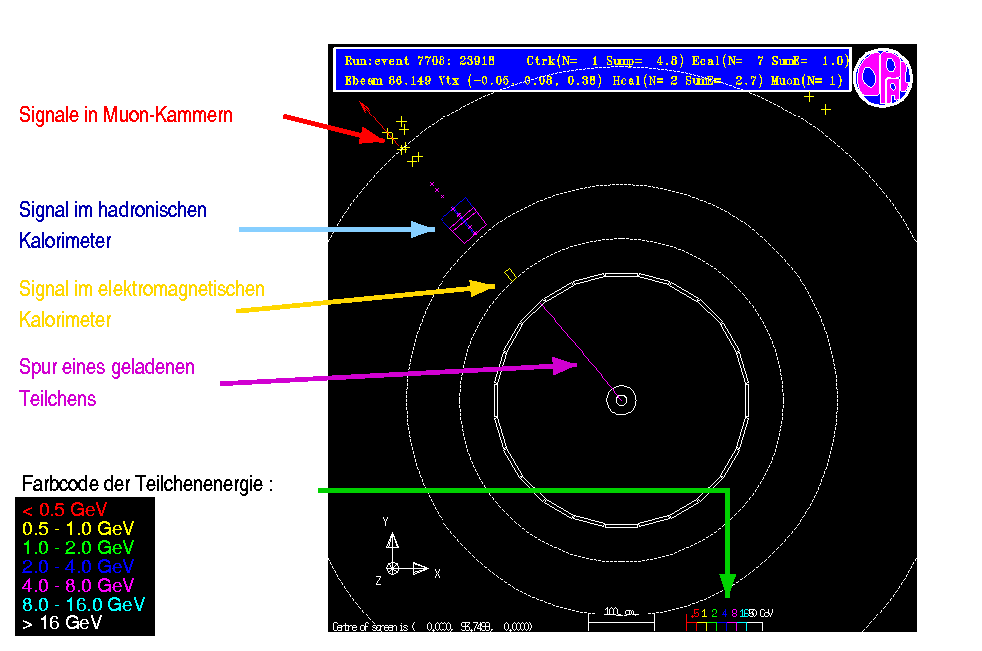
\includegraphics[width=\textwidth]{opalevents/ex_all}
       \vskip0.2cm
       \begin{columns}
         \begin{column}{0.05\textwidth}
         \end{column}
         \begin{column}{0.9\textwidth}
           \begin{block}{$\znull\rightarrow \tau^{+}\tau^{-}$}
             \begin{itemize}
             \item Je $e$ oder $\mu$ oder Jet (1$h$ oder 3$h$)
             \end{itemize}
           \end{block}
         \end{column}
         \begin{column}{0.05\textwidth}
         \end{column}
       \end{columns}
     \end{column}
  \end{columns}
 \end{frame}
